% This file was created by tikzplotlib v0.9.8.
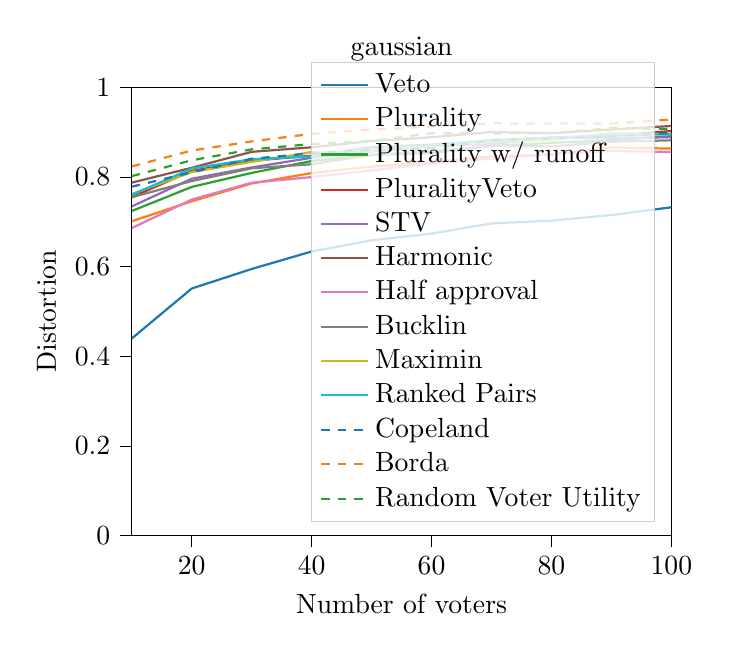
\begin{tikzpicture}

\definecolor{color0}{rgb}{0.12156862745098,0.466666666666667,0.705882352941177}
\definecolor{color1}{rgb}{1,0.498039215686275,0.0549019607843137}
\definecolor{color2}{rgb}{0.172549019607843,0.627450980392157,0.172549019607843}
\definecolor{color3}{rgb}{0.83921568627451,0.152941176470588,0.156862745098039}
\definecolor{color4}{rgb}{0.580392156862745,0.403921568627451,0.741176470588235}
\definecolor{color5}{rgb}{0.549019607843137,0.337254901960784,0.294117647058824}
\definecolor{color6}{rgb}{0.890196078431372,0.466666666666667,0.76078431372549}
\definecolor{color7}{rgb}{0.737254901960784,0.741176470588235,0.133333333333333}
\definecolor{color8}{rgb}{0.0901960784313725,0.745098039215686,0.811764705882353}

\begin{axis}[
legend cell align={left},
legend style={
  fill opacity=0.8,
  draw opacity=1,
  text opacity=1,
  at={(0.97,0.03)},
  anchor=south east,
  draw=white!80!black
},
tick align=outside,
tick pos=left,
title={gaussian},
x grid style={white!69.0196078431373!black},
xlabel={Number of voters},
xmin=10, xmax=100,
xtick style={color=black},
y grid style={white!69.0196078431373!black},
ylabel={Distortion},
ymin=0, ymax=1,
ytick style={color=black}
]
\addplot [thick, color0]
table {%
10 0.4393
20 0.5508
30 0.5944
40 0.6334
50 0.6583
60 0.6733
70 0.696
80 0.7022
90 0.7147
100 0.732
};
\addlegendentry{Veto}
\addplot [thick, color1]
table {%
10 0.7009
20 0.7453
30 0.7852
40 0.8083
50 0.8229
60 0.8315
70 0.8458
80 0.849
90 0.8653
100 0.8629
};
\addlegendentry{Plurality}
\addplot [thick, color2]
table {%
10 0.7237
20 0.7774
30 0.8087
40 0.8352
50 0.8488
60 0.8528
70 0.8689
80 0.8757
90 0.8817
100 0.8907
};
\addlegendentry{Plurality w/ runoff}
\addplot [thick, color3]
table {%
10 0.7546
20 0.8132
30 0.8357
40 0.8471
50 0.8659
60 0.8717
70 0.881
80 0.8876
90 0.8915
100 0.9021
};
\addlegendentry{PluralityVeto}
\addplot [thick, color4]
table {%
10 0.7339
20 0.7957
30 0.8209
40 0.8424
50 0.8562
60 0.8692
70 0.8728
80 0.8869
90 0.8865
100 0.8883
};
\addlegendentry{STV}
\addplot [thick, color5]
table {%
10 0.787
20 0.8201
30 0.8557
40 0.8658
50 0.8796
60 0.8883
70 0.8998
80 0.8974
90 0.9054
100 0.9134
};
\addlegendentry{Harmonic}
\addplot [thick, color6]
table {%
10 0.6856
20 0.7492
30 0.7868
40 0.7994
50 0.8142
60 0.8298
70 0.8407
80 0.8509
90 0.8576
100 0.8553
};
\addlegendentry{Half approval}
\addplot [thick, white!49.8039215686275!black]
table {%
10 0.7544
20 0.7905
30 0.819
40 0.828
50 0.8489
60 0.8569
70 0.8686
80 0.8678
90 0.8781
100 0.8814
};
\addlegendentry{Bucklin}
\addplot [thick, color7]
table {%
10 0.7616
20 0.8105
30 0.8332
40 0.8552
50 0.8577
60 0.8677
70 0.8776
80 0.8824
90 0.8976
100 0.8947
};
\addlegendentry{Maximin}
\addplot [thick, color8]
table {%
10 0.7596
20 0.8185
30 0.8393
40 0.8453
50 0.8641
60 0.8698
70 0.8825
80 0.8867
90 0.8923
100 0.8951
};
\addlegendentry{Ranked Pairs}
\addplot [thick, color0, dashed]
table {%
10 0.7779
20 0.8101
30 0.8402
40 0.8525
50 0.8597
60 0.8631
70 0.8812
80 0.8854
90 0.89
100 0.8979
};
\addlegendentry{Copeland}
\addplot [thick, color1, dashed]
table {%
10 0.8232
20 0.8586
30 0.879
40 0.8958
50 0.9052
60 0.9122
70 0.9193
80 0.9187
90 0.919
100 0.9278
};
\addlegendentry{Borda}
\addplot [thick, color2, dashed]
table {%
10 0.8015
20 0.8369
30 0.8612
40 0.873
50 0.8802
60 0.8973
70 0.8968
80 0.8969
90 0.9087
100 0.9065
};
\addlegendentry{Random Voter Utility}
\end{axis}

\end{tikzpicture}
